\section{Appendix}
\subsection{Magnetic shims drawing}
\label{magnetic shims}

The following figures illustrate the design specifications of the magnetic shims used in the magnet units. These shims are critical in fine-tuning the magnetic field distribution within the units. Figure \ref{fig:mu16_shim} and Figure \ref{fig:mu16_shim2} depict the magnetic shim for magnet unit 016, showing the top and side views. Similarly, Figure \ref{fig:mu63_shim} and Figure \ref{fig:mu63_shim2} present the magnetic shim for magnet unit 063.

\begin{figure}[h]
    \centering
    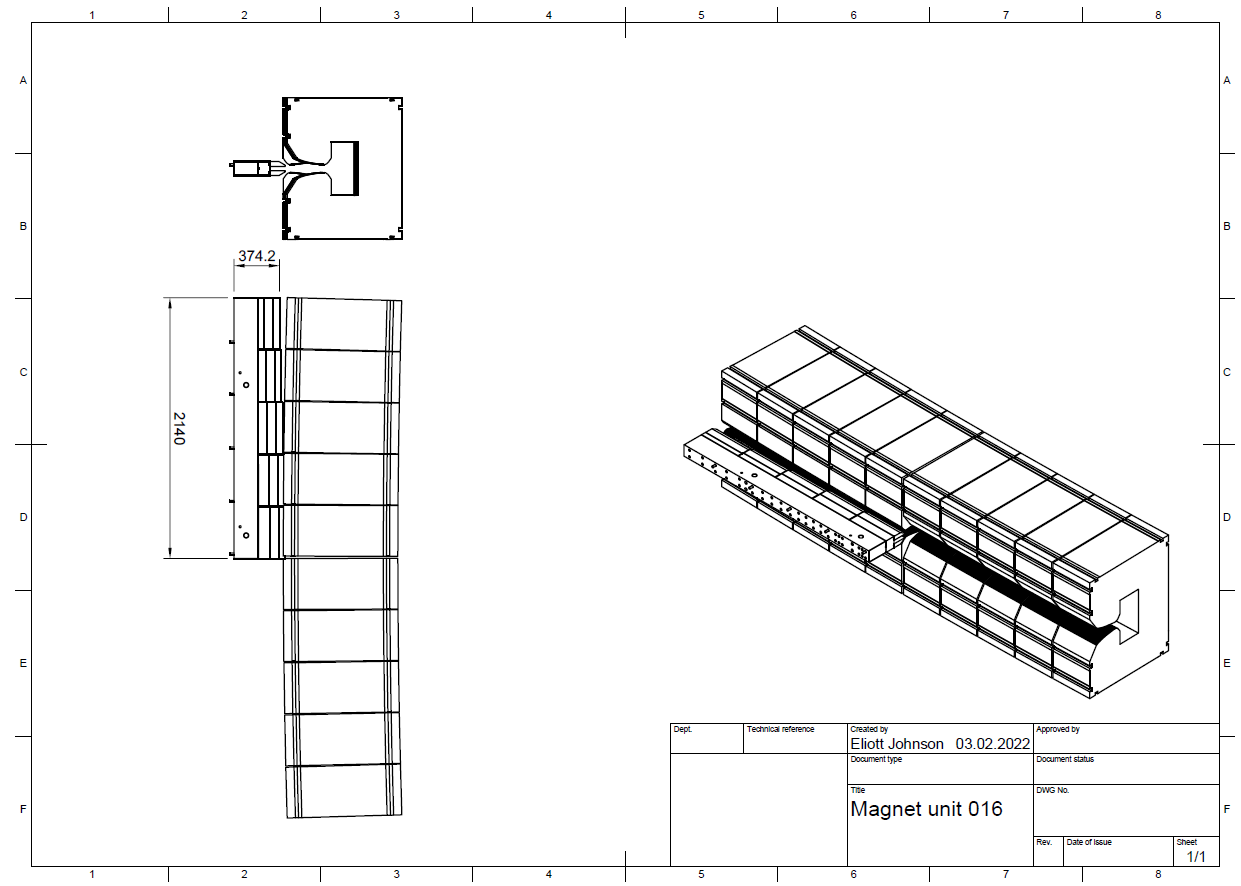
\includegraphics[width=1.0\textwidth]{Appendix/images/mu16_shim.png}
    \caption{Magnetic shim for main unit 016.}
    \label{fig:mu16_shim}
\end{figure}

\begin{figure}[h]
    \centering
    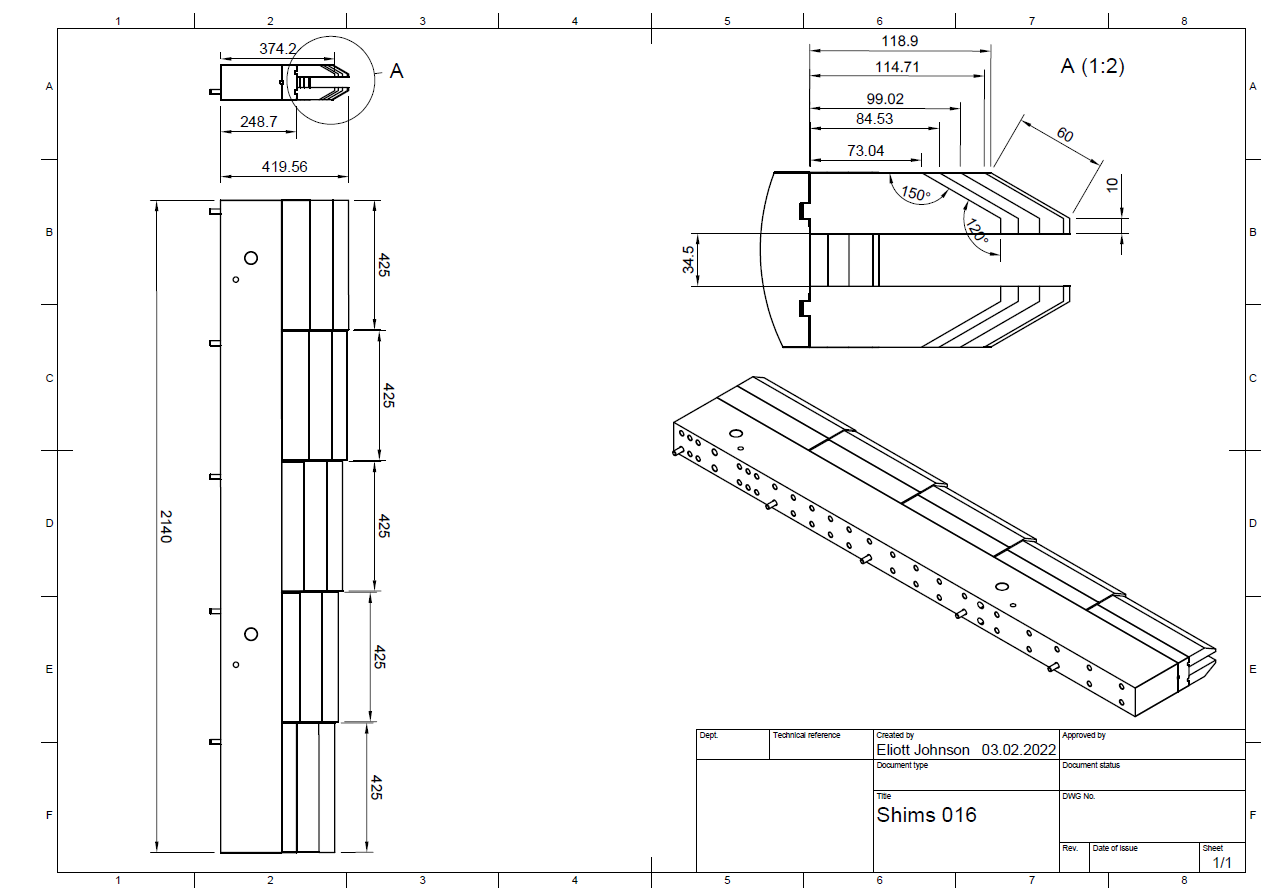
\includegraphics[width=1.0\textwidth]{Appendix/images/mu16_shim2.png}
    \caption{Magnetic shim for main unit 016.}
    \label{fig:mu16_shim2}
\end{figure}

\begin{figure}[h]
    \centering
    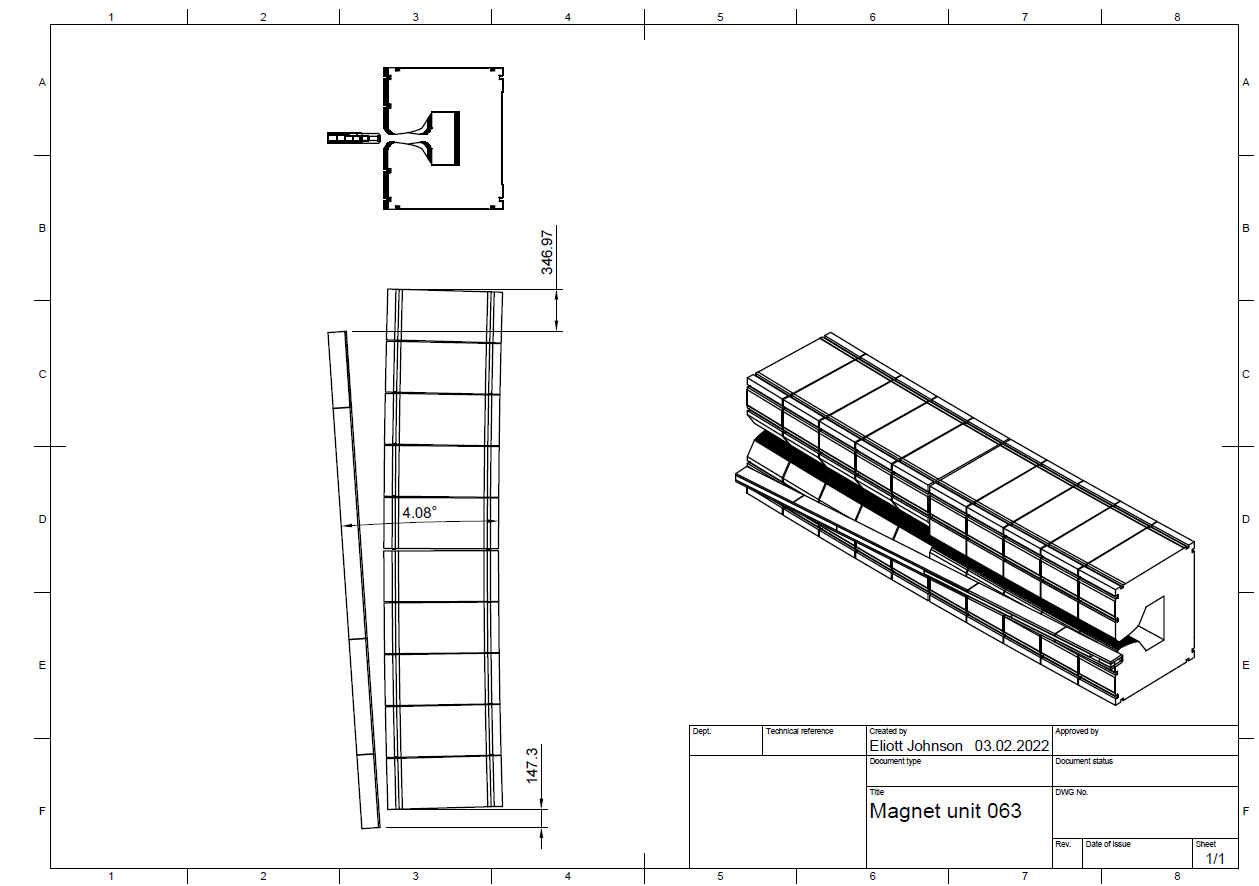
\includegraphics[width=1.0\textwidth]{Appendix/images/mu63_shim.png}
    \caption{Magnetic shim for main unit 063.}
    \label{fig:mu63_shim}
\end{figure}

\begin{figure}[h]
    \centering
    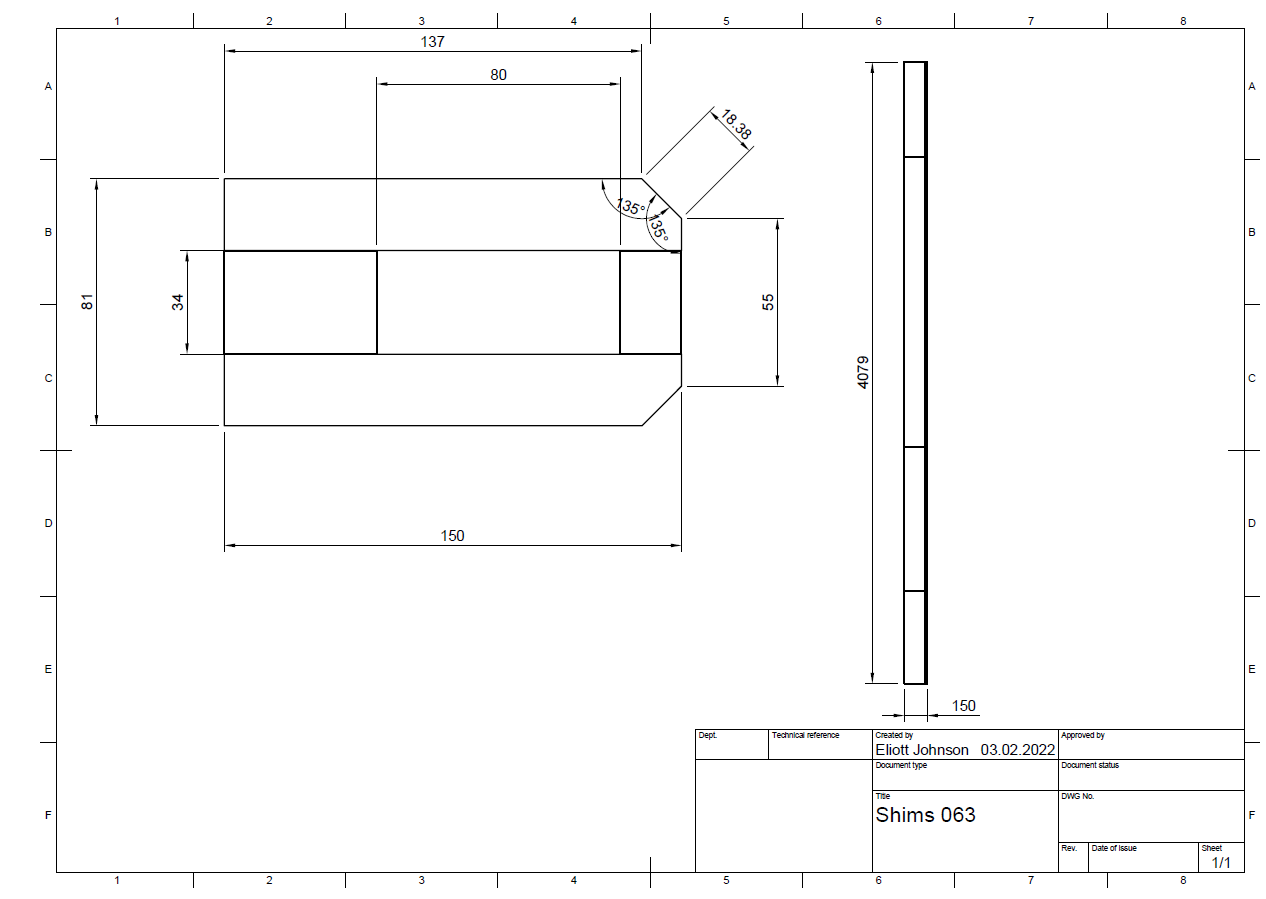
\includegraphics[width=1.0\textwidth]{Appendix/images/mu63_shim2.png}
    \caption{Magnetic shim for main unit 063.}
    \label{fig:mu63_shim2}
\end{figure}

\begin{figure}[h]
    \centering
    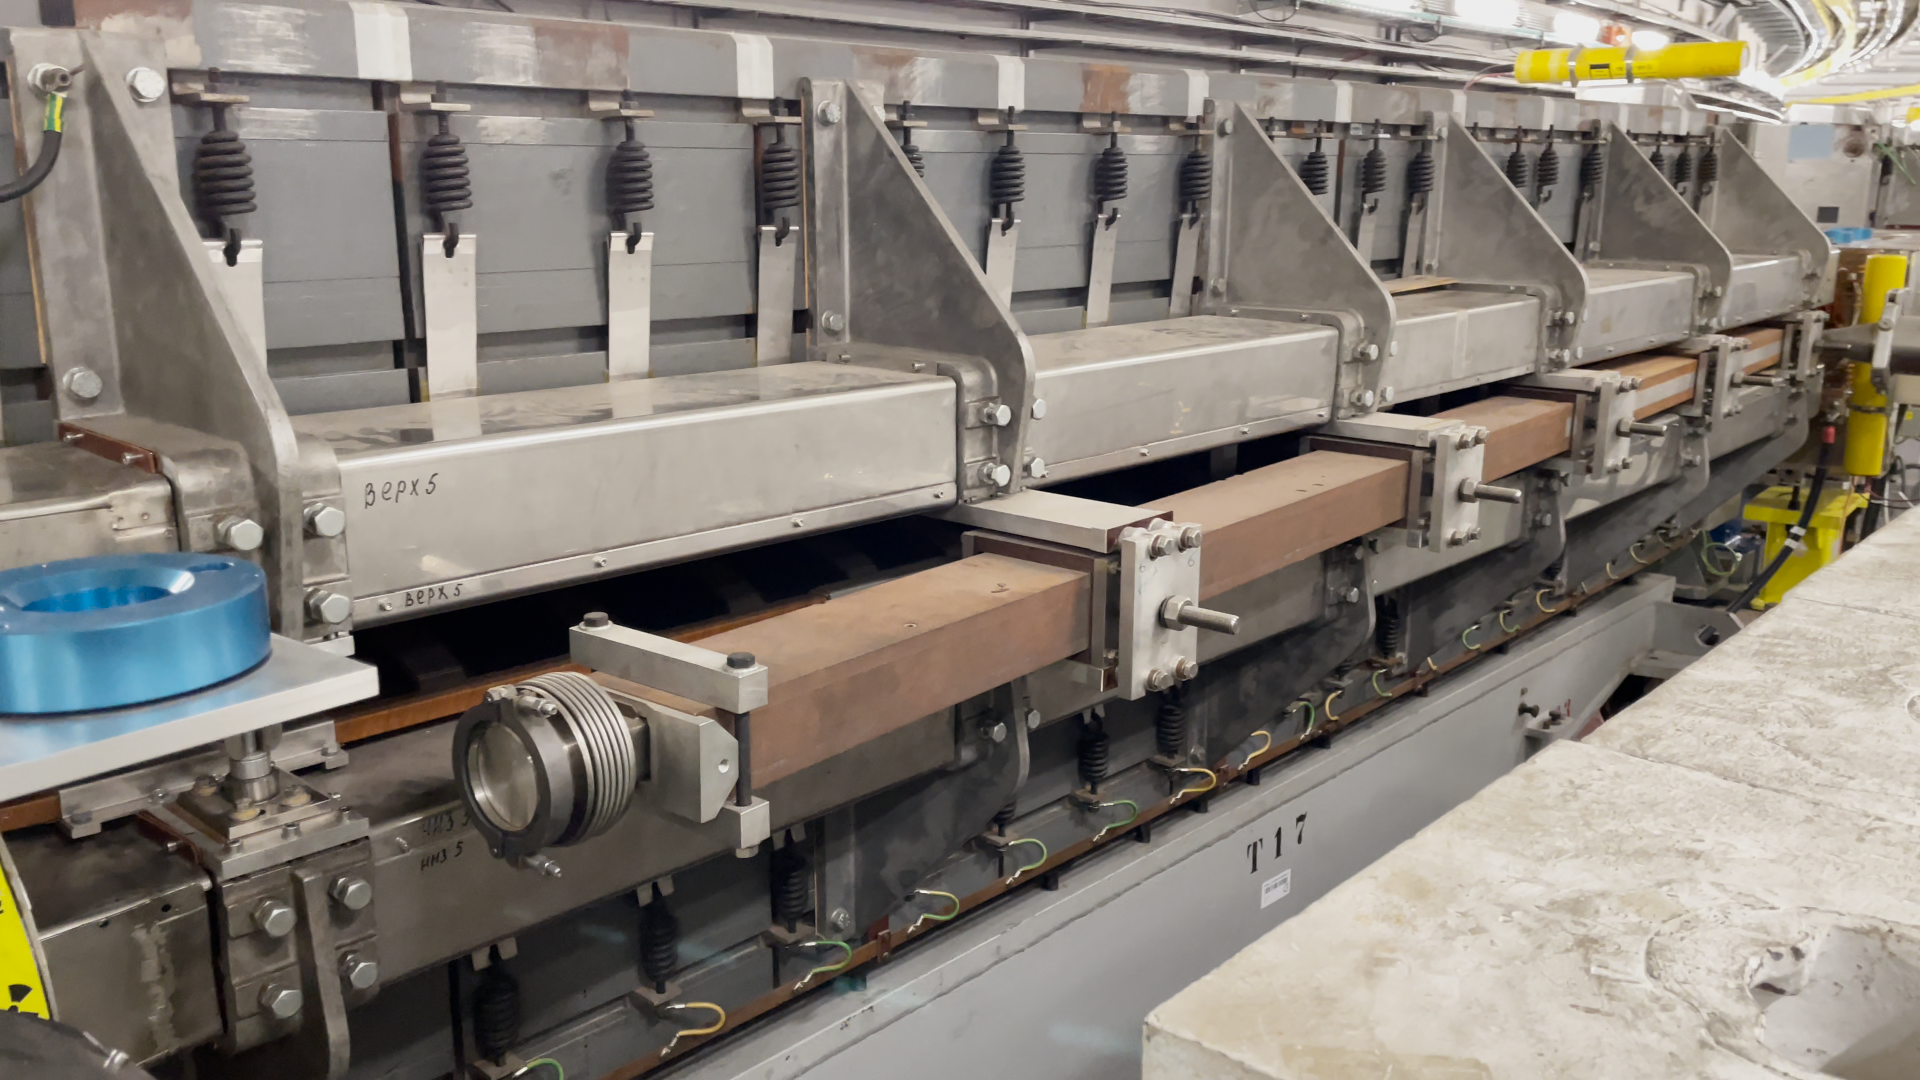
\includegraphics[width=1.0\textwidth]{Appendix/images/mu63_shim3.png}
    \caption{Picture of MU63.}
    \label{fig:mu63_shim3}
\end{figure}

The magnetic shim in MU41, see Fig. \ref{fig:mu41_shim}, constructed from mu-metal (SCEM 44.72.60.005.6) characterized by its high permeability, are crucial components in maintaining the stability of the magnetic field within the injection main unit. These shims have a thickness of 0.5 mm and undergo a heat treatment process at 1070°C to enhance their magnetic properties. This mu metal is designed to overlap by 10° on each side, typically oriented on the top and bottom for ease of installation, although alternative orientations are feasible.

The vacuum pipe, fabricated from 316LN stainless steel, was a point of curiosity for Jose due to its magnetic properties when combined with mu-metal. Despite Jose not being directly involved in the project, he noted the interesting choice of 316LN, a low magnetic permeable material. This material allows magnetic field lines to pass through without significant distortion, thereby limiting the perturbation of the charged particle beam as it travels through the beam transport tube. This design ensures minimal interference with the beam's trajectory, maintaining the precision required for successful particle acceleration.


\begin{figure}[h]
    \centering
    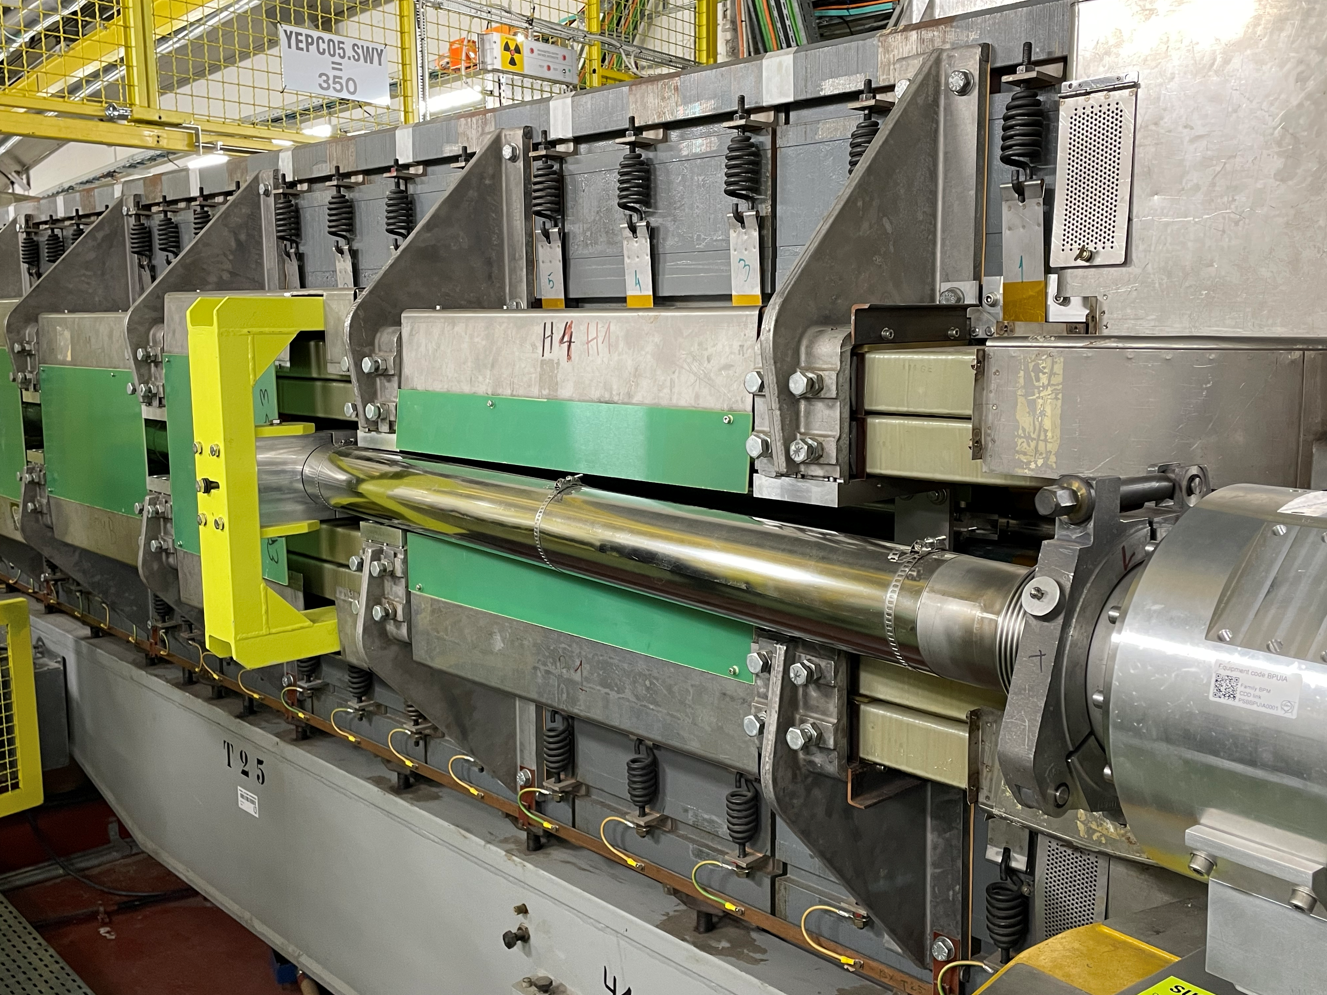
\includegraphics[width=1.0\textwidth]{Appendix/images/mu41_shim.png}
    \caption{MU41 - Injection in the PS with mu metal shielding.}
    \label{fig:mu41_shim}
\end{figure}